%!TEX root = /Users/high/Documents/School/Thesis/report/thesis.tex

\section{Architecture} % (fold)
\label{sec:arch}

In this section, a description of the overall architecture that are used in the implementation of the PRiDe protocol will be explained in more detail. The PRiDe implementation will be referred as Evaluation PRiDe (EPRiDe) for the remaining of the report.  

% (end)

\subsection{Concepts} % (fold)
\label{sub:consepts}

In an application that uses replication to increase availability, we establish a distinction between \emph{local objects} and \emph{database objects}. Local objects are temporary objects that the application uses but there is no need to store these objects permanently. Database objects are objects that are used in the application and are durable, which means that the object can't be lost if any error occurs. To increase fault tolerance for database objects, these objects are replicated to other nodes so that if the node crashes, the information is stored on at least one more node. 

A database object is associated with a unique database object identifier(DBOID) that is unique between all EPRiDe nodes in the network. This is means any logical object in a EPRiDe instance can't have the same identifier as another object on the same EPRiDe instance or on any other instance in the network.    

A database object can store primitive data types. This includes for example int, char, double. Pointer to other database objects are not handled and are out of scope for this implementation. One possible solution is to define a interface that has a number of operations that are handled by EPRiDe and are mapped to objects that executes the actual methods.  

A database object can only read and write data. Each read operation are not allowed to change the internal state of the database object. Database objects are not allowed to send messages to other database objects since these messages can create inconsistency between replicas in the network.

To be able to store updates that are performed on database object, EPRiDe logs each operation that is performed on the database object including parameters. This type of logging is referred as \emph{operational logging}. Operational logging increases the semantics used in conflict resolution compared to value logging, where only the result of the operation are logged. 


% (end)

%\subsection{Transactions} % (fold)
%\label{sub:transactions}

%Transaction
%	Identified by an ID
	
%	Transaction contains a number of operations. These operations can be both read and write operations. 
%	A transaction can only have operations that affect one object. (Own subchapter?)
	
%	Each transaction are send as one segment to the conflict set with one generation Id.
%	The transaction stores a tentative object where all operations have been performed. 
	
%	Each transaction are not removed from the transaction store until the transaction have been stabilized with a conflict resolution routine.  

%Transactions is PRiDe 
%	In PRiDe, only on transaction is allowed at the time. when a transaction is replicated, the transaction is not isolated from concurrent updates that have been performed on another PRiDe instance. This means that when a transaction, containing updates u1 to u3 on node N1 have been commited, and propagated, another concurrent update u4 that where performed on N2, are in conflict with u2. Then when the conflict resolution decides that it throws away the update u2, then the transaction isolation is broken. 
	


% subsection transactions (end)

\subsection{Components} % (fold)
\label{sub:components}

Each EPRiDe instance consists of a number of components:

\begin{description}
	\item[Application] \
		The application component is responsible for handling read and write requests that an application can make. This includes transaction commands.
		
	\item[Propagater] \
		The propagater is responsible for sending updates that are in the conflict set to the other EPRiDe instances. The propagater is used  when a commit has been performed on the node and the information needs to be replicated to the other EPRiDe instances.
		
	\item[Receiver] \
		This component receives propagation messages that are send from other EPRiDe nodes. The receiver receives each message, unpacks the message and puts the information into the correct generation.
		
	\item[Stabilizater] \
		This component performs stabilization on a generation with a specified conflict resolution routine that have been configured beforehand.
\end{description}

% subsection components (end)

\subsection{Data structures} % (fold)
\label{sub:datastructures}

The components in the EPRiDe architecture uses a number of data structures to store conflicts, transaction information and object state. 
\begin{description}
	
	\item[Transaction Store] \
	is responsible for storing information about a transaction that the application creates. Each transaction is stored in a separate database file in Berkeley DB.  Each transaction file stores which operations that have been performed in the transaction. A transaction can only handle operations that are for a specific object.
	
	\item[Conflict Set] \
	stores each update generation in a list that is created when an operation is performed on a database object. The update generation list is ordered on generation identifier. A generation identifier is defined as the age of the object on the specific replica and is represented with a number \cite[]{Syber2007}.
	
	Each generation in the conflict set, contains state information for each replica \cite[]{Syber2007}. There are three different types of states: \emph{Update}, \emph{No\_update} and \emph{None}. Update means that the replica has an update on the specific generation. No\_update means that there where no updates on that specific generation on the replica. None means that the replica has not given any information about the specific generation. 
	
	\item[Object Store] stores the stable version of all database objects. When a generation has been considered stable by a conflict resolution policy, the actions that have been decided are conducted on the stable object.
	
\end{description}
     
% subsection datastructures (end)

\subsection{Data interaction} % (fold)
\label{sub:data_interaction}

Figure \ref{fig:components} illustrates the components, the defined data structures and their interactions. 

\begin{figure}[htb]
\centerline{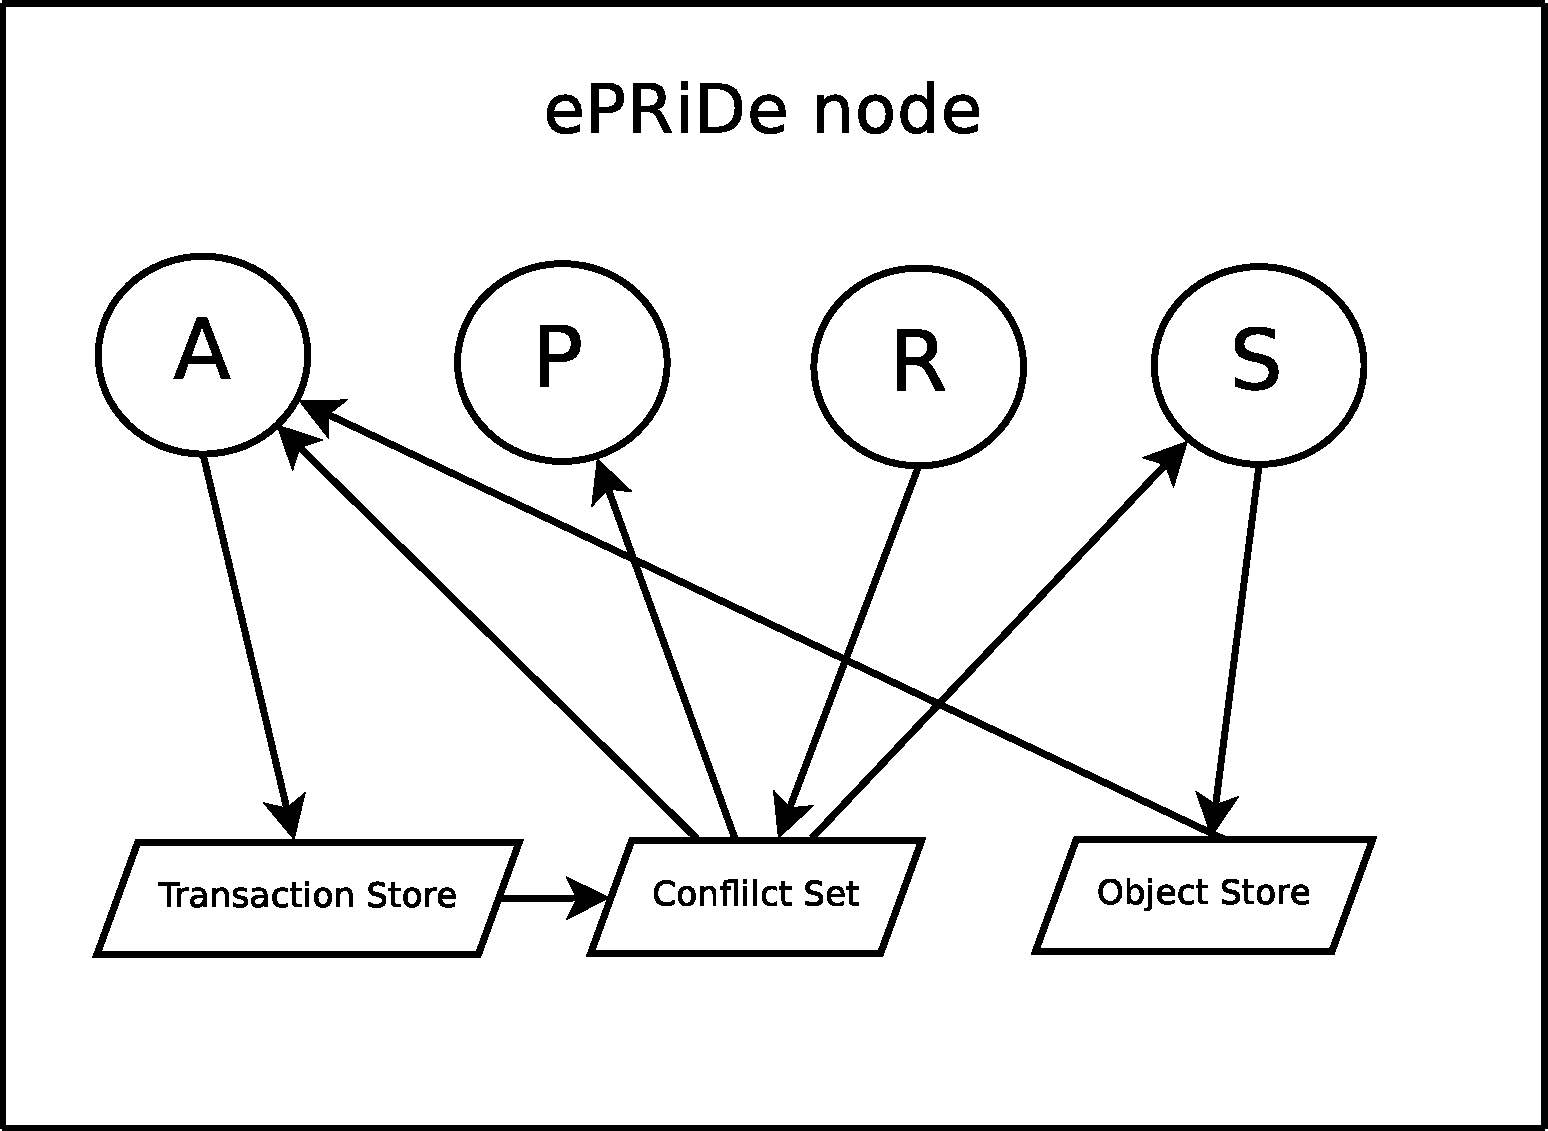
\includegraphics[height=8cm]{components.pdf}}
\caption{The components used in EPRiDe and their interactions}\label{fig:components}
\end{figure}


When a application wants to write to the object, the method call is logged and registered inside the transaction store. The transaction stores the operation and the new state of the object after the operation has been performed. When a commit is called by the application, the transaction containing all operations are send to the conflict set and each write operations creates a new generation. Each generation that is created are propagated to the other EPRiDe nodes in the network. 

When a propagation is received by the reciever, the update is stored in the objects conflict set and are given the highest generation id plus one. Each generation that has a lower generation id than the generation id that was generated, are set to No\_update for the given replica. 

Stabilization is performed on a defined interval of 2 seconds. During this event, one generation are stabilized using a defined conflict resolution routine. The result that the conflict resolution routine decides, are applied to the stable object that is stored in the object store.
  


When an application process want to read a stable object, the read routine fetches the object state from the object store. If the application process wants to read a optimistic object, the following tasks are performed: 
\begin{enumerate}
	\item A stable version of the object are fetched from the object store.
	\item If there are any generations in the conflict set for the given object, these are resolved by the Stabilizater. The Stabilizater stabilizates each generation by perfoming a conflict resolution routine on each generation. 
	\item Each generation that is stabilized, the outcome of the conflict resolution are performed on the object. 
	\item The read process returns the optimistic object after each unstable update have been performed.
\end{enumerate}

\subsection{Implementation} % (fold)
\label{sub:implementation}

(((( Describe details about the implementation, what software, programming language etc. ))))
% subsection implementation (end)

% subsection data_interaction (end)

%(fold)

%Each EPRiDe instance contains a number of components:
% 	- Application 
% 		This component is responsible for handling read and write requests that an application can make. This includes transaction commands. 
%
%	- Propagater
%		The propagater is responsible for sending updates that are in the conflict set to the other EPRiDe instances. The propagater is used  when a commit has been performed on the node and the informmation needs to be replicated to the other EPRiDe instances.

%	- Receiver 
%		This component receives propagation messages that are send from other EPRiDe nodes. The receiver receives each message, unpacks the message and puts the information into the correct generation.

%	- Stabilizater 
%		This component performs stabilization on each generation when needed. 

% To be able to serve these components, a number of datastructures are used. A transaction store are used by the application to store transaction informantion. This information contains the operations that have been conducted inside the transaction and the object state with each operation. This is similar to a write-ahead log [ref here]. A conflict set is used to handle the different generation on a specific object. 

% - Describe replication 
% - Describe each module
% 	- Why, when 
%		- Application 
%		- Receiver 
%		- Propagater
%		- Stabilizator
%	
% - Describe the flow in number of activity diagrams
% (end)
